\documentclass{report}
\usepackage[utf8]{inputenc}
\usepackage{graphicx}
\usepackage{tabularx}
\usepackage{listings}
\usepackage{float}
\usepackage[siunitx,europeanresistors,americaninductors]{circuitikz}
\usepackage{pgfplots}
\usepackage[
	colorlinks=true,
	urlcolor=blue,
	linkcolor=violet
]{hyperref}
\title{Report on Laboratory work 2}
\author{Elisabeth Kretschmer}
\date{March 21st 2018}

\begin{document}

\chapter{Theoretical part}

\section{Circuit calculation} \label{circuit calculation}
For the theoretical calculation of the circuit (Laboratory Work~01, circuit diagram given in figure \ref{circuit}), I calculated the voltages on the resistors within the given circuit. My student ID is 181ADM007. According to the instructions given in the document P01\_EN.pdf, the following voltage of the voltage source $V_1$ and resistances $R_1$ and $R_2$ were assumed:
\[V_1=0.07\ V\]
\[R_1=1\ \Omega\]
\[R_2=8\ \Omega\]
\\
For the voltages on the resistors, the following formulas were applied:
\[U_{R1}=\frac{R_1}{R_1+R_2}\ V_1\]
\[U_{R2}=\frac{R_2}{R_1+R_2}\ V_1\]
\\
Hence, the voltages on the resistors have the following values:
\[U_{R1}=\frac{1\ \Omega}{1\ \Omega+8\ \Omega}\ 0.07\ V=0.00\overline{7}\ V\]
\[U_{R2}=\frac{8\ \Omega}{1\ \Omega+8\ \Omega}\ 0.07\ V=0.06\overline{2}\ V\]
\\
For an overview over all values see table \ref{values}. 

\begin{figure}
    \centering
    \begin{circuitikz}
\draw
(0,0) to [european resistor, l=$R_1$ ] (6,0)
to [european resistor, l=$R_2$] (6,-4)
to [short, *-] (0,-4)
to [battery1, l=$V_1$] (0,0)
;
\end{circuitikz}
    \caption{Circuit diagram}
    \label{circuit}
\end{figure}

\begin{table}
    \centering
    \begin{tabular}{ |c|c| }
    \hline
$V_1$ & 1\ V \\
\hline
$R_1$ & 1\ \Omega \\
\hline
$R_2$ & 8\ \Omega \\
\hline
$U_{R1}$ & 0.00\overline{7}\ V \\
\hline
$U_{R2}$ & 0.06\overline{2}\ V \\
\hline
    \end{tabular}
    \caption{Values of circuit calculation}
    \label{values}
\end{table}

\begin{figure}[!b]
    \centering
    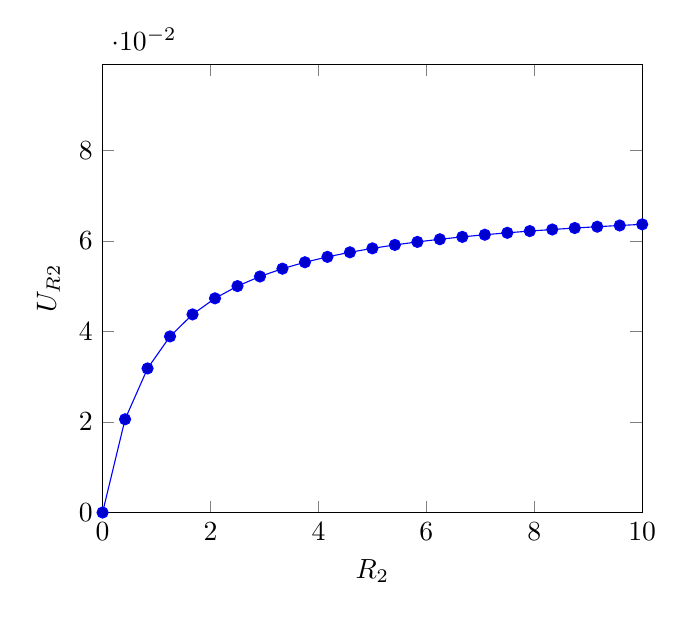
\begin{tikzpicture}
\begin{axis}[ xlabel=$R_2$, ylabel=$U_{R2}$, xmin=0, xmax=10, ymin=0, ymax=0.099, domain=0:10]
\addplot {x/(1+x)*0.07};
\end{axis}
\end{tikzpicture}
    \caption{Plot of $U_{R2}$ as function of $R_2$}
    \label{U_R2 plot}
\end{figure}

\chapter{Practical part}

\section{Work with GEDA programs}

\subsection{Work with gschem}

\begin{figure}[H]
    \centering
    \rotatebox{-90}{
    \includegraphics[width=10cm]{01.ps}}
     \caption{Image of gschem schematics}
    \label{gschem}
\end{figure}

\subsection{Work with gnetlist}
% insert contents of 01.net using lstinputlisting
\lstinputlisting{01.net}

\subsection{Work with ngspice}

\begin{figure}[h]
    \centering
    \includegraphics[width=\textwidth]{11.png}
     \caption{Plot of R1 simulation}
    \label{R1}
\end{figure}
\begin{figure}[H]
    \centering
    \includegraphics[width=\textwidth]{12.png}
     \caption{Plot of R2 simulation}
    \label{R2}
\end{figure}

\section{Work with QUCS programs}
For the DC simulation with QUCS, I first created the schematics of the circuit with the same properties as used for the gEDA modeling (according to the theoretical calculation in section \ref{circuit calculation}). The QUCS schematics as well as the DC simulation plot can be found in figures \ref{schematics} and \ref{sim}, respectively.
\begin{figure}[t]
    \centering
    \includegraphics[width=\textwidth]{P01QUCSschematics.png}
    \caption{Image of QUCS schematics}
    \label{schematics}
\end{figure}

\begin{figure}[t]
    \centering
    \includegraphics[width=\textwidth]{P01QUCSsimresults.png}
    \caption{Plot of DC simulation.}
    \label{sim}
\end{figure}

\section{Work with \LaTeX}
This document was created on \url{http://sharelatex.com}. The laboratory works within this Computer Studies course were my first experience working with this document preparation system. I found the ShareLaTeX guide \cite{web1} to be very helpful. A book that was also recommended by many for learning to work with \LaTeX is The \LaTeX Companion \cite{book1}.
\begin{thebibliography}{9}
\bibitem{web1}
“Documentation.” ShareLaTeX, 2018. Web. March 21st 2018. \\
URL: \texttt{https://www.sharelatex.com/learn}
\bibitem{book1}
"The \LaTeX Companion, Second Edition." Frank Mittelbach and Michael Goossens. Addison-Wesley, 2004.
\end{thebibliography}

\end{document}

